\subsection{系统开发环境}

FoodShield 系统采用轻量化 Web 原型方式实现，后端基于 Python Flask 框架构建 HTTP 接口和 WebSocket 通信服务，前端采用 HTML、CSS 和 JavaScript 实现用户端、骑手端和管理员端页面，数据库采用 SQLite 存储用户、订单、通信消息和审计日志数据。系统整体开发和测试均在本地环境完成，便于快速迭代、联调和演示。

系统主要开发环境如表~\ref{tab:dev-env} 所示。

\begin{table}[H]
    \centering
    \caption{FoodShield 系统开发环境}
    \label{tab:dev-env}
    \begin{tabular}{p{4cm}p{8cm}}
        \toprule
        项目 & 配置 \\
        \midrule
        操作系统 & Windows 11 \\
        开发工具 & Visual Studio Code \\
        后端语言 & Python 3.x \\
        后端框架 & Flask、Flask-SocketIO \\
        数据库 & SQLite \\
        前端技术 & HTML、CSS、JavaScript \\
        通信机制 & WebSocket \\
        密码算法 & HMAC-SM3、SM3、SM4-CBC \\
        运行方式 & \texttt{python -m project.server.app} \\
        访问地址 & \texttt{http://127.0.0.1:5000} \\
        \bottomrule
    \end{tabular}
\end{table}

系统启动时，后端首先执行数据库初始化操作，检查 \texttt{users}、\texttt{orders}、\texttt{messages} 和 \texttt{audit\_logs} 等核心数据表是否存在。若数据表不存在，则自动创建相关表结构；若数据表已存在，则直接加载现有数据并启动服务。启动完成后，Flask 服务监听本地 5000 端口，用户可通过浏览器访问用户端、骑手端和管理员端页面。

\begin{figure}[H]
    \centering
    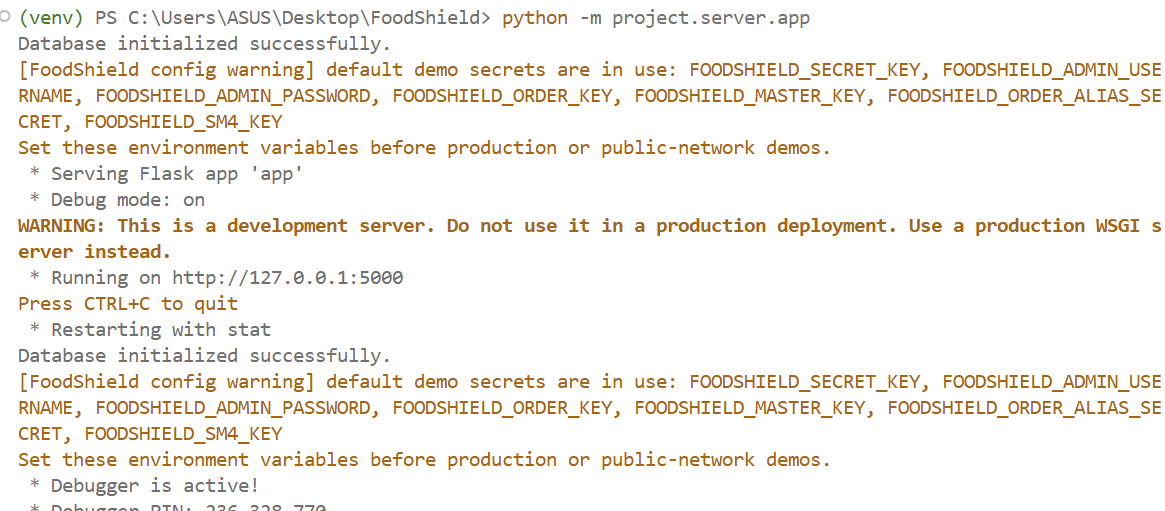
\includegraphics[width=0.95\textwidth]{content/chapter4/backend_start.png}
    \caption{系统后端服务启动界面}
    \label{fig:backend-start}
\end{figure}
